\clearpage
\chapter{System design}\label{ch:design}
\begingroup
\clubpenalty=10000
\widowpenalty=10000
\brokenpenalty=10000

\section{Representing the patient state}

We use a patient state to connect MRI observations to anatomical predictions. The state needs to retain current anatomy in a form that a temporal model can use. We assess these requirements separately: anatomical readouts show what can be recovered from the state, while forecasting tests what it can predict about a later visit.

The compact JEPA branch encodes each visit as a feature vector and predicts the features of a later visit. Readouts convert those features into compartment volumes. The spatial branch retains feature maps and decodes masks as well as volumes, giving the decoder direct access to spatial information. Figure~\ref{fig:4.1} shows how the two representations connect observed MRI to future targets.

\begin{figure}[!htbp]\centering
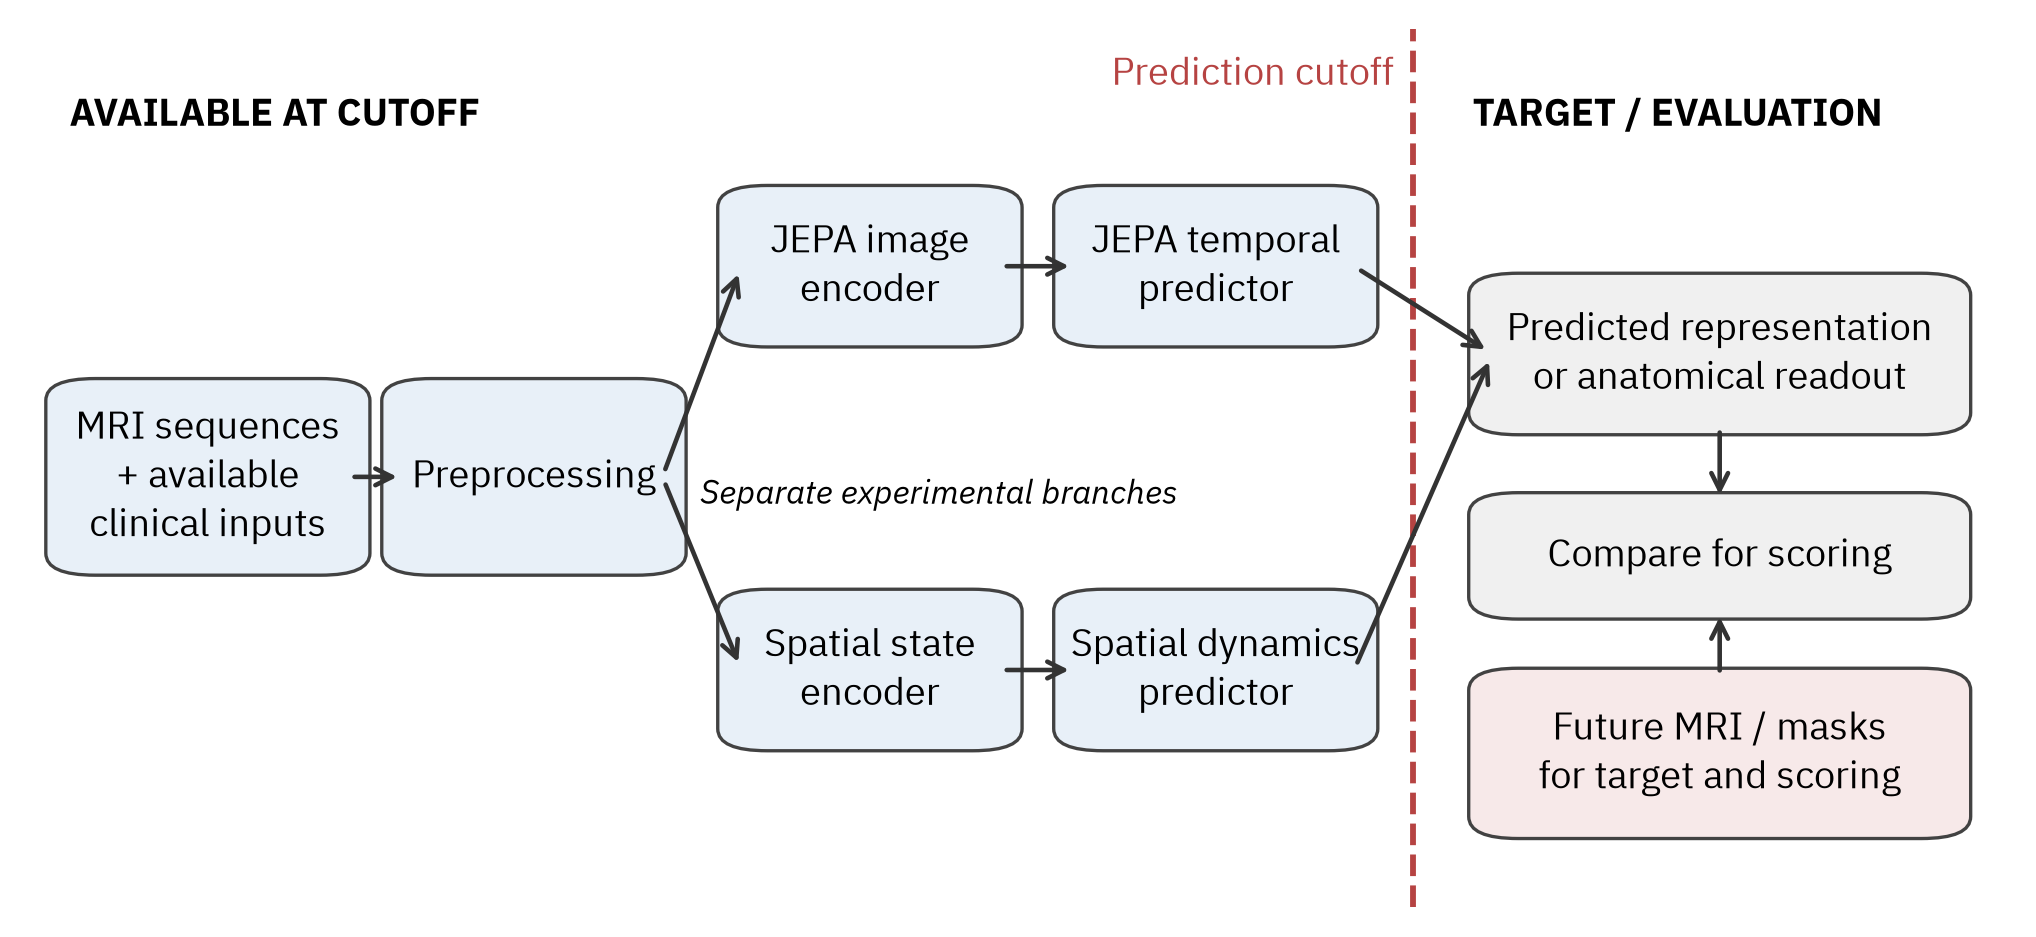
\includegraphics[width=\linewidth,height=0.57\textheight,keepaspectratio]{figures/figure_4_1.png}
\caption[Image-based experimental branches]{JEPA and spatial-state forecasting branches. Observed MRI forms the input; later MRI and masks provide targets for learning and evaluation.}\label{fig:4.1}
\end{figure}

\section{MRI inputs and anatomical supervision}\label{sec:cohorts}

The input sequences are T1, contrast-enhanced T1 (CT1), T2 and fluid-attenuated inversion recovery (FLAIR). Sequence-availability flags accompany the images so that the encoder can distinguish a missing sequence from an observed image with low intensity. Visits retain their order and past intervals when they enter a temporal model.

LUMIERE and SAILOR provide longitudinal MRI with automated anatomical references from DeepBraTumIA and ONCOHabitats respectively. Their compartments cover enhancing tumor, necrotic or nonenhancing tissue, and edema or FLAIR abnormality. MU-Glioma-Post provides neuroradiologist-reviewed masks with a separate resection-cavity label. These masks define the anatomical targets for the readouts.

Mask supervision gives the spatial encoder information about tissue location and boundaries. Volume supervision ties its features to anatomical burden. We measure physical volumes from the source segmentation and its voxel-to-world transform, before resizing masks for the network. For regional prediction, each labeled source voxel contributes its volume to one of eight fixed regions according to its center. This avoids losing small labeled structures through downsampling.

Cavity supervision gives the integrated observation model five output categories: background, enhancing tumor, nonenhancing core, FLAIR abnormality and cavity. LUMIERE has no cavity annotation, so its anatomical loss uses the four annotated categories. We evaluate both a conditional readout that removes the cavity logit and the native five-category readout. This makes the effect of the extra output category visible when comparing anatomical predictions.

\section{Learning from partial observations}

Missing-sequence completion gives us another way to test what the state retains. The model predicts withheld current FLAIR from the available sequences. Comparing CT1 alone with CT1 plus T1, and then with CT1 plus T1 and T2, tests the information added by each sequence. Giving the decoder higher-resolution spatial features tests whether it can use information that a compact state may lose.

A new readout fitted to a frozen state tests whether those features remain useful for another anatomical task. For segmentation, frozen random features and direct-image adaptation provide references for learned information and the cost of fixing the representation. The integrated observation model supports both anatomical decoding and missing-sequence completion from the same saved state.

History-assisted completion asks a related question about the present: whether a previous scan helps recover current FLAIR. Current images alone, genuine patient history and timing-matched donor history distinguish the contribution of the patient's own earlier observations. Registered previous-FLAIR persistence provides a reference for how much can be recovered simply by retaining the previous image.

\section{Forecasting from the observed state}\label{sec:cutoff}

A history model receives the current state and eligible earlier states, together with past timing. In the spatial branch, a recurrent predictor combines the feature maps and predicts a correction to the latest state. Its anatomical decoder maps the predicted features to future volumes. We also fit forecasts directly to measured volumes and previous measured change. This makes it possible to test the value of history without requiring an MRI encoder to recover those measurements first.

The main control is a matched latest-only model. It receives the current MRI state and the same timing and availability information, with earlier MRI features removed. For numerical volume models, the corresponding current-only control omits previous measured change. Matching the remaining inputs makes the comparison depend on the historical information being tested.

Persistence supplies a second reference by copying current anatomy to the target visit. Measured-volume persistence uses volumes from a current mask; decoded-state persistence uses the model's estimates from current MRI. The latter shares the state-estimation error of an MRI-based forecast. A latest-only predictor can improve on persistence, so the history comparison is needed to establish whether earlier visits add anything. Figure~\ref{fig:4.2} shows the information available on each side of the prediction cutoff.

\begin{figure}[!htbp]\centering
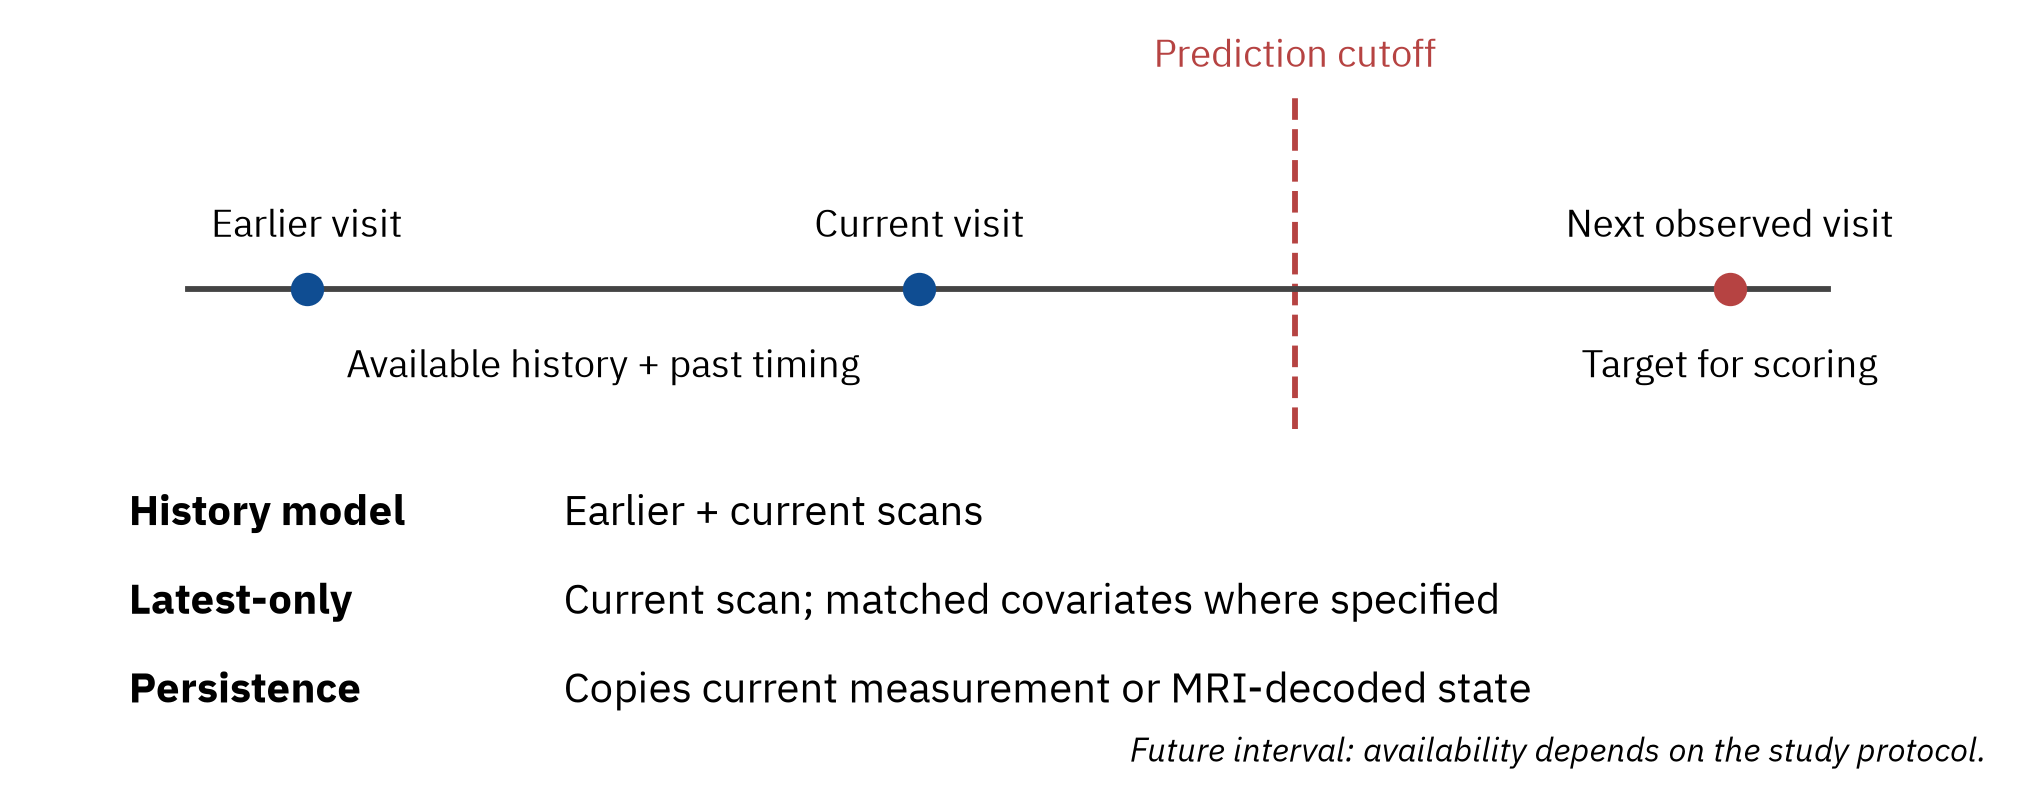
\includegraphics[width=\linewidth,height=0.57\textheight,keepaspectratio]{figures/figure_4_2.png}
\caption[Forecast inputs and comparison baselines]{History and latest-only predictors share the current observation. Persistence copies current anatomy, and the later observation supplies the target.}\label{fig:4.2}
\end{figure}

Next-visit models predict the next scan without knowing its interval in advance. Horizon-conditioned models receive an interval: the structured forecasts use requested horizons of 12 or 24 weeks, while retrospective comparisons supply the actual follow-up gap. LUMIERE intervals use nominal week bins; MU intervals use recorded days.

Completion can also prepare a representation for forecasting. We freeze the completion-adapted and original encoders and fit fresh matched history and latest-only heads to each. Both heads can use the latest observed FLAIR. This tests whether better recovery of a current image carries over to prediction of a later one.

Structured forecasts describe future anatomy through multiple anatomical scenarios. Compartment presence, amount and spatial allocation determine each scenario, with volumes computed from its segmentation. This keeps the predicted shape and burden consistent within a scenario. Quantity models isolate presence and amount before introducing spatial allocation: an accurate-looking boundary would be of limited use if the model predicted the wrong amount of tissue. Scalar-volume controls test whether MRI features add predictive information beyond current anatomical measurements. Recorded treatment status can also enter as an additional covariate in a matched forecast comparison.

\section{Choosing another MRI sequence}

The state also supports a choice about what to observe next. Starting with T1, the acquisition model chooses which available sequence to reveal. The JEPA selector uses predicted features of a candidate sequence alongside the observed state; the direct selector uses the observed state alone. Once the chosen MRI is revealed, it updates the state.

We compare both selectors with a fixed acquisition order at budgets of two and three observed sequences. Their utility is the anatomical score at those budgets, so a useful choice must improve the state available for anatomical prediction. An oracle that chooses using target outcomes estimates how much improvement is available under the same observer. This separates the quality of the selection rule from the observer's ability to benefit from an additional sequence.

\section{Evaluation design}\label{sec:evaluation}

The comparisons follow the role of each component. Current-state tests assess anatomical recovery, forecast tests assess later anatomy, and acquisition tests assess the value of another observation. Table~\ref{tab:4.1} summarizes the main questions and the controls that make them interpretable.

\begin{table}[!htbp]\centering
\singlespacing\small\setlength{\tabcolsep}{4pt}\renewcommand{\arraystretch}{1.2}
\caption[Design questions and matched comparisons]{Design questions, matched comparisons and anatomical endpoints.}\label{tab:4.1}
\begin{tabular}{>{\raggedright\arraybackslash}p{\dimexpr 0.25\linewidth-2\tabcolsep\relax}>{\raggedright\arraybackslash}p{\dimexpr 0.46\linewidth-2\tabcolsep\relax}>{\raggedright\arraybackslash}p{\dimexpr 0.29\linewidth-2\tabcolsep\relax}}
\toprule \textbf{Question} & \textbf{Comparison} & \textbf{Endpoint} \\\midrule
Does initialization help? & Pretrained and random encoders with matched architecture and supervision & Current masks and volumes \\
Does spatial access help? & Higher-resolution decoder features enabled or zeroed & Current FLAIR and local image detail \\
Does history help forecasting? & History versus latest-only or current-only, with persistence as a reference & Future anatomy and volume distributions \\
Does history help completion? & Current images alone, genuine history and donor history & Withheld current FLAIR \\
Does sequence selection help? & JEPA selector, direct selector and fixed order & Anatomy after two and three sequences \\
\bottomrule
\end{tabular}
\end{table}

Mean absolute error (MAE) scores a point prediction, while the continuous ranked probability score (CRPS) scores a predictive distribution. Lower is better for both. Dice measures segmentation overlap from zero to one. Empty and nonempty reference compartments are reported separately where required, since predicting absence and recovering the shape of present tissue are different tasks.

The volume endpoint depends on the model. Whole-compartment regression comparisons use log1p(mm³), the logarithm of one plus numerical volume in cubic millimetres. Corrected regional forecasts use log1p(mL), and structured and quantity forecasts score volumes in mL. Image errors use standardized intensity. We compare models on the same target and scale, rather than ranking absolute errors across these endpoints.

For scenario forecasts, Dice scores the weighted vote of the segmentations and volume MAE scores the distribution mean. A displayed scenario is one possible output. The final quantity comparisons compute core mean-volume and CRPS scores from the fitted discrete distribution, avoiding dependence on a small scenario sample.

Patients contribute different numbers of visits, so we average eligible observations within each patient before averaging across patients. Multi-seed results average scores from separately fitted models; repeated-partition comparisons average their partition scores. Paired bootstrap intervals resample patients while keeping competing predictions together. We judge a gain through its size and uncertainty, alongside consistency across patients and fitted models. The task-specific scoring definitions and decision criteria are given in the methods \cite{record}, with paired results in Chapter~\ref{ch:results}.

\endgroup
